---
name: State Machine
category: diagrams
description: Finite automaton with states and transitions using TikZ automata library
packages:
  - tikz
preamble:
  - \usetikzlibrary{automata,positioning,arrows.meta}
---
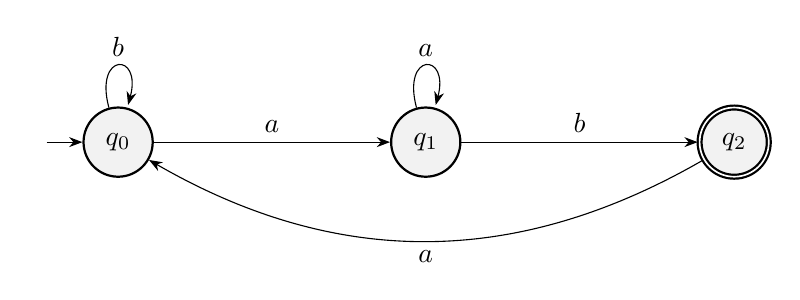
\begin{tikzpicture}[
  ->,
  >=Stealth,
  node distance=3cm,
  every state/.style={thick, fill=gray!10},
  initial text={},
]
  \node[state, initial]           (q0) {$q_0$};
  \node[state, right=of q0]      (q1) {$q_1$};
  \node[state, accepting, right=of q1] (q2) {$q_2$};

  \path (q0) edge[above]       node{$a$} (q1)
             edge[loop above]  node{$b$} ()
        (q1) edge[above]       node{$b$} (q2)
             edge[loop above]  node{$a$} ()
        (q2) edge[bend left, below] node{$a$} (q0);
\end{tikzpicture}
